%%%%%%%%%%%%%%%%%%%%%%%%%%%%%%%%%%%%%%
%         PACKAGES INCLUSION         %                                                                                      % PACKAGES
%%%%%%%%%%%%%%%%%%%%%%%%%%%%%%%%%%%%%%

\documentclass[a4paper,10pt]{article}                                                                                       % Document specs
\usepackage[legalpaper, margin=2cm]{geometry}                                                                               % Document margin
\usepackage[italian]{babel}                                                                                                 % Document language
\usepackage{tocloft}                                                                                                        % Package import for table of contents with dots
\usepackage{abstract}                                                                                                       % Package import for abstract
\usepackage{hyperref}                                                                                                       % Package import for external references
\usepackage{graphicx}                                                                                                       % Package import to manage images labels and captions
\usepackage{float}                                                                                                          % Package import to manage tables and images positioning
\usepackage{url}                                                                                                            % Package import for links
\usepackage{cite}                                                                                                           % Package import for bibliographies (citations)
\usepackage[usenames,dvipsnames,svgnames,table]{xcolor}                                                                     % Package import for colors
\usepackage{amsmath}                                                                                                        % Package import for formulas (math)
\usepackage{amssymb}                                                                                                        % Package import for formulas (symbols)
\usepackage{chngcntr}                                                                                                       % Package import for formulas (enumeration)

%%%%%%%%%%%%%%%%%%%%%%%%%%%%%%%%%%%%%%
%           PREAMBLE START           %                                                                                      % PREAMBLE
%%%%%%%%%%%%%%%%%%%%%%%%%%%%%%%%%%%%%%

\hypersetup{
  colorlinks=true,
  linkcolor=darkgray,
  filecolor=magenta,
  urlcolor=blue,
  citecolor=gray,
  pdftitle={DataAnalysis},
  pdfpagemode=FullScreen}                                                                                                   % External references definition: dark-grey links and blue URLs (\href call)
\setlength{\parindent}{1cm}                                                                                                 % Remove indentation at paragraph's start
\renewcommand{\cftsecleader}{\cftdotfill{\cftdotsep}}                                                                       % Configure table of contents (ToC) to display dots
\renewcommand{\cftsecfont}{\normalsize}                                                                                     % ToC-sec font
\renewcommand{\cftsubsecfont}{\normalsize}                                                                                  % ToC-subsec font
\renewcommand{\cftsubsubsecfont}{\normalsize}                                                                               % ToC-subsubsec font
\setlength{\cftsecindent}{0mm}                                                                                              % ToC-sec indentation
\setlength{\cftsubsecindent}{2mm}                                                                                           % ToC-subsec indentation
\setlength{\cftsubsubsecindent}{4mm}                                                                                        % ToC-subsubsec indentation
\setlength{\cftsecnumwidth}{5mm}                                                                                            % ToC-sec distance from number
\setlength{\cftsubsecnumwidth}{8mm}                                                                                         % ToC-subsec distance from number
\setlength{\cftsubsubsecnumwidth}{11mm}                                                                                     % ToC-subsubsec distance from number
\renewcommand{\theequation}{{Eq.} \thesubsubsection.\arabic{equation}}                                                      % Change equations enumeration
\counterwithin*{equation}{section}                                                                                          % Restart equations enumeration at new section
\counterwithin*{equation}{subsection}                                                                                       % Restart equations enumeration at new subsection
\counterwithin*{equation}{subsubsection}                                                                                    % Restart equations enumeration at new subsubsection
\bibliographystyle{plain}                                                                                                   % Bibliography style (plain standard style)

\title{Analisi dati e calcoli ingegneristici scambiatore di calore\\                                                        % Title definition (printed with \maketitle command)
\large Laboratorio - Gruppo n.5 del 26/11/2021, fisica tecnica [140078] AA 2021/2022}                                       % Subtitle definition (printed with \maketitle command)
\author{Cristian Merli, mat. 211384}                                                                                        % Authors definition (printed with \maketitle command)
\date{07/02/2022}                                                                                                           % Date definition (printed with \maketitle command)

%%%%%%%%%%%%%%%%%%%%%%%%%%%%%%%%%%%%%%
% END OF PREAMBLE and DOCUMENT START %                                                                                      % DOC-START
%%%%%%%%%%%%%%%%%%%%%%%%%%%%%%%%%%%%%%

\begin{document}                                                                                                            % Document-start

\maketitle                                                                                                                  % Plot previously defined title
\vspace{5cm}                                                                                                                % Vertical-space command
\addcontentsline{toc}{section}{Sommario}                                                                                    % Add abstract inside table of contents
\begin{abstract}                                                                                                            % Abstract creation and following abstract text
  \noindent \textit{Relazione con lo scopo di descrivere le scelte adottate, e discutere i risultati  ottenuti dall'analisi
  dati e dalle modellazioni ingegneristiche effettuate. Il sistema oggetto di modellazione, è costituito da uno scambiatore
  di calore a fascio tubiero, all'interno del quale scorre acqua in entrambi i circuiti di scambio. Sono state effettuate
  diverse prove, in particolare: due in configurazione equi-corrente e due in configurazione contro-corrente, con diversi
  valori di portata volumetrica di fluido freddo.\\
  Nei capitoli successivi, verranno elencate le richieste di progetto avanzate dal docente e verranno ripercorse le varie
  tappe, che hanno condotto alla realizzazione e comparazione di diversi modelli ingegneristici più o meno raffinati,
  mediante l'analisi assistita da calcolatore dei dati raccolti durante l'esperienza di laboratorio (effettuata in data
  26/11/2021 con il gruppo numero 5, presso i laboratori del dipartimento di fisica dell'università di Trento).}
\end{abstract}                                                                                                              % Abstract end
\pagebreak                                                                                                                  % Go to new page

\tableofcontents                                                                                                            % Plot table of contents
\vspace{1.5cm}                                                                                                              % Vertical-space command
\listoftables                                                                                                               % Plot list of tables
\vspace{1.5cm}                                                                                                              % Vertical-space command
\listoffigures                                                                                                              % Plot listo of figures
\pagebreak                                                                                                                  % Go to new page

\section{Richieste}                                                                                                         % Section creation: "Richieste"
\label{sec:project_request}                                                                                                 % "project_request" reference-label definition and following section text
  Le richieste di progetto consistono principalmente nella realizzazione di un sistema di analisi dati "computerizzato",
  per poter cogliere da esso, le informazioni necessarie ad effettuare i diversi calcoli inerenti il fenomeno di scambio
  termico. Il tutto, con l'obiettivo di caratterizzare tale fenomeno sul manufatto oggetto di analisi sperimentale. In
  aggiunta, è stato richiesto di identificare le analogie e tutto ciò in cui i risultati teorici attesi, differiscono da
  quelli sperimentali ottenuti, con particolare attenzione in riferimento alla non adiabaticità del sistema e alle varie
  approssimazioni effettuate in fase di modellazione, per lo studio del trasferimento di calore all'interno e all'esterno
  della macchina termica.

\section{Introduzione}                                                                                                      % Section creation: "Introduzione"
\label{sec:introduction}                                                                                                    % "introduction" reference-label definition and following section text
  Per rispondere alle richieste di progetto, come riportato anche nel sommario di questo documento, è stata
  realizzata una parte di calcolo assistito con alcuni commenti per motivare e descrivere i vari passaggi effettuati.
  Questo elaborato ha quindi come unico scopo, quello di illustrare i passaggi cruciali, le scelte salienti adottate e
  discutere i risultati ottenuti nella parte tecnica. Per maggior trasparenza, è stato reso accessibile online l'intero
  codice sorgente realizzato, senza la necessità di effettuare alcuna installazione e/o configurazione dell'ambiente di
  sviluppo per poterlo consultare. Il seguente link, consente un accesso diretto alla repository di GitHub caricata
  personalmente, per poter approfondire tutto ciò che è stato realizzato:
  \textit{\href{https://github.com/CristianMerli/DataAnalysis.git}{https://github.com/CristianMerli/DataAnalysis.git}} .

\section{Linguaggio di programmazione}                                                                                      % Section creation: "Linguaggio di programmazione"
\label{sec:progr_lang}                                                                                                      % "progr_lang" reference-label definition and following section text
  Il passo preliminare per poter portare a compimento le richieste avanzate da parte del docente
  \textit{\textbf{[}\hyperref[sec:project_request]{Capitolo }\ref{sec:project_request},
  \hyperref[sec:project_request]{pagina }\pageref{sec:project_request}\textbf{]}}, è stato quello di
  individuare un software di "data science", per la realizzazione della parte di analisi dati e calcolo ingegneristico.
  La scelta più ovvia in ambito accademico, sarebbe stata quella di utilizzare il software MatLab, ma si è optato per un
  programma di tipo open-source, riutilizzabile anche in futuro essendo libero da licenze. É stato quindi scelto un
  linguaggio denominato python, dotato di numerosi pacchetti dedicati al "data science", tra cui pandas e numpy.
  L'ambiente di sviluppo utilizzato (IDE) è Visual Studio Code, installato su una macchina linux con un ambiente virtuale
  python dedicato allo sviluppo di tale progetto (conda environment). Un esempio di configurazione simile per analisi
  dati, può essere trovato al seguente link:
  \textit{\href{https://code.visualstudio.com/docs/datascience/data-science-tutorial}{vedi esempio}}. Infine, è stato
  utilizzato il sistema di gestione del codice "git", unitamente al servizio di hosting fornito da GitHub, con l'intento
  di pubblicare online e rendere facilmente accessibili tutti i contenuti realizzati. Il codice che compone la parte
  tecnica di questo progetto, è composto da uno script python principale di tipo JupyterNotebook e da un pacchetto
  (libreria) appositamente sviluppato, denominato "libs". Esso contiene diversi script in linguaggio nativo python, con
  compiti specifici tra cui: caricamento dati misure, esecuzione analisi dati, formule di calcolo ingegneristico,
  stampaggio a video di grafici, approssimazione polinomiale delle proprietà delle variabili termofisiche e molto
  altro.\vspace{2mm}\\
  "One of the really big growth areas for Python is in the sciences, where data analysis is a huge component."
  \textit{(by Bernard, Joey)}
  \cite{Bernard2016}

\section{Analisi dati}                                                                                                      % Section creation: "Analisi dati"
\label{sec:data_analysis}                                                                                                   % "data_analysis" reference-label definition and following section text
\subsection{Fase preliminare}                                                                                               % Subsection creation: "Fase preliminare"
\label{subsec:prelim_phase}                                                                                                 % "prelim_phase" reference-label definition and following subsection text  
  Per prima cosa, dopo aver auto-inizializzato l'ambiente, il codice esegue delle operazioni preliminari prima di
  procedere con l'analisi dati vera e propria. In sequenza, il file contenente le misure sperimentali, viene caricato e
  rielaborato dal software creando un file CSV appositamente formattato
  (\textit{\href{https://github.com/CristianMerli/DataAnalysis/blob/master/data_analysis/dataset/scambiatore26112021_5.dat}{file-DAT}},
  \textit{\href{https://github.com/CristianMerli/DataAnalysis/blob/master/data_analysis/dataset/scambiatore26112021_5.csv}{file-CSV}}).
  Quest'ultimo, a sua volta convertito in un database, viene utilizzato come sorgente dati da cui attingere al fine di
  estrapolare informazioni, per compiere operazioni di filtraggio e di calcolo. Il programma, identifica quindi in maniera
  autonoma le diverse misure all'interno del database, ripulendo inoltre ulteriori eventuali dati intermedi corrispondenti
  ad "altre operazioni". Il tutto viene poi mostrato graficamente, evidenziando le finestre dati corrispondenti alle
  misure stesse \textit{\textbf{[}\hyperref[fig:measures]{Fig. }\ref{fig:measures}\textbf{]}}.
\subsection{Definizione valori e creazione strutture dati}                                                                  % Subsection creation: "Definizione valori e creazione strutture dati"
\label{subsec:valsdef_datastruct}                                                                                           % "valsdef_datastruct" reference-label definition and following subsection text  
  Conclusa questa fase preparativa, vengono automaticamente richiamate le istruzioni per compiere l'analisi dati vera e
  propria. Tali istruzioni hanno come scopo principale, quello di ottenere i valori numerici delle diverse variabili
  misurate, per ogni misura: temperature e portate volumetriche. Il tutto, cercando di ricavare valori numerici
  significativi, per poter successivamente svolgere i calcoli ingegneristici richiesti. In particolare, essendo le
  equazioni utilizzate valide sotto condizioni di stazionarietà, il software sceglie intervalli dati che soddisfino
  al meglio tali requisiti. Nello specifico, ciò avviene mediante l'implementazione informatica dell'equazione
  \textit{\textbf{[}\ref{eqn:stat}\textbf{]}}, utilizzata per identificare gli intervalli dati, da cui ricavare il valore
  medio delle variabili rilevate sperimentalmente. Anche in questo caso le operazioni vengono rappresentate graficamente,
  come mostrato ad esempio per la prima misura in
  \textit{\textbf{[}\hyperref[fig:measure1]{Fig. }\ref{fig:measure1}\textbf{]}}, dove viene evidenziato l'intervallo
  selezionato. Vengono quindi creati in maniera autonoma, degli oggetti informatici di tipo "misura", i quali ne
  conterranno tutte le informazioni. In fase di creazione della lista di oggetti "misura", ne viene auto-determinata la
  tipologia (equi-corrente o contro-corrente) in base al testo di descrizione, e vengono popolate le variabili
  corrispondenti ai valori delle misure, riportati anche nella tabella dedicata:
  \textit{\textbf{[}\hyperref[tab:measures_data]{Tab. }\ref{tab:measures_data}\textbf{]}}. Questi oggetti, hanno inoltre
  lo scopo di contenere tutti i risultati dei calcoli ingegneristici raggruppati per misura, in modo da poter essere
  facilmente richiamati nelle formule di calcolo e poter essere stampati a video o esportati su file, in maniera rapida
  e ordinata.\vspace{2mm}\\
  \textit{Nota:} i file esportati dallo script principale di calcolo, possono essere consultati al seguente
  \textit{\href{https://github.com/CristianMerli/DataAnalysis/tree/master/final_doc/code_exports/output}{link}}.

\section{Calcoli ingegneristici}                                                                                            % Section creation: "Calcoli ingegneristici"
\label{sec:engineering_calcs}                                                                                               % "engineering_calcs" reference-label definition and following section text
\subsection{Approssimazione polinomiale variabili termofisiche}                                                             % Subsection creation: "Approssimazione polinomiale variabili termofisiche"
\label{subsec:thermovars_polyapprox}                                                                                        % "thermovars_polyapprox" reference-label definition and following subsection text  
  Al fine di ottenere risultati il più possibile veritieri, anche le variabili termofisiche dei materiali/fluidi
  costituenti o interagenti con l'apparato di scambio termico, sono state approssimate polinomialmente in funzione della
  temperatura. I dati di partenza utilizzati per approssimare l'andamento delle diverse proprietà con la temperatura,
  derivano da fonti ufficiali ed affidabili. Nel dettaglio, i dati riguardanti i fluidi: aria ed acqua, sono stati forniti
  dal docente sotto forma di tabelle (pdf), poi trascritte in file CSV ed importate sotto forma di database. Procedura
  analoga, anche per i materiali costituenti lo scambiatore: acciaio inox AISI-316 (tubi interni) e vetro borosilicato
  (pyrex, tubo esterno), i cui dati derivano però dalla rete. Di seguito, sono riportate nel dettaglio le fonti dati
  utilizzate:
  \begin{itemize}                                                                                                           % List-start
    \item \textbf{proprietà aria a pressione atmosferica:}
      prima tabella all'interno del file pdf
      (\textit{\href{https://github.com/CristianMerli/DataAnalysis/blob/master/lab_doc/TabelleAriaAcqua.pdf}{file-PDF}},
      \textit{\href{https://github.com/CristianMerli/DataAnalysis/blob/master/data_analysis/thermophys_vars/air_atmp_thermo_vars.csv}{file-CSV}}).
    \item \textbf{proprietà acqua:}
      seconda tabella all'interno del file pdf
      (\textit{\href{https://github.com/CristianMerli/DataAnalysis/blob/master/lab_doc/TabelleAriaAcqua.pdf}{file-PDF}},
      \textit{\href{https://github.com/CristianMerli/DataAnalysis/blob/master/data_analysis/thermophys_vars/water_thermo_vars.csv}{file-CSV}}).
    \item \textbf{proprietà AISI-316:}
      \textit{\href{http://www.inductor-jmag.ru/files/content/a129160.pdf}{http://www.inductor-jmag.ru/files/content/a129160.pdf}}
      pagina 28 pdf, tabella 4 (pagina 21 file)
      (\textit{\href{https://github.com/CristianMerli/DataAnalysis/blob/master/lab_doc/AISI316.pdf}{file-PDF}},
      \textit{\href{https://github.com/CristianMerli/DataAnalysis/blob/master/data_analysis/thermophys_vars/aisi_316_thermo_vars.csv}{file-CSV}}).
      \vspace{1.5mm}\\\textit{Nota:} le temperature sono state convertite da [K] a [°C], all'interno dello script dedicato
      all'approssimazione delle proprietà termofisiche.
    \item \textbf{proprietà vetro pyrex:}
      \textit{\href{https://nvlpubs.nist.gov/nistpubs/Legacy/RPT/nbsreport7836.pdf}{https://nvlpubs.nist.gov/nistpubs/Legacy/RPT/nbsreport7836.pdf}}
      pagina 39 pdf, tabella 6 (pagina 16 file)
      (\textit{\href{https://github.com/CristianMerli/DataAnalysis/blob/master/lab_doc/Pyrex_glass.pdf}{file-PDF}},
      \textit{\href{https://github.com/CristianMerli/DataAnalysis/blob/master/data_analysis/thermophys_vars/pyrex_glass_thermo_vars.csv}{file-CSV}}).
      \vspace{1.5mm}\\\textit{Nota:} i valori della conducibilità termica, sono stati convertiti da [W/(cm\*K)] a
      [W/(m\*K)], all'interno dello script dedicato
      \vspace{1.5mm}\\\textit{Nota:} in caso d'errore in fase di caricamento dell'anteprima file PDF, dovuto alle
      dimensioni eccessive del file stesso, premere il pulsante "download", oppure usa il seguente
      \textit{\href{https://github.com/CristianMerli/DataAnalysis/raw/master/lab_doc/Pyrex_glass.pdf}{link}}).
  \end{itemize}                                                                                                             % List-end
  Questi dati, sono quindi la base su cui uno script appositamente sviluppato, esegue operazioni di approssimazione
  polinomiale mediante interpolazione o "curve-fitting". Dopo di che, caso per caso, viene scelto il metodo che meglio
  definisce l'andamento del grafico. Anche queste operazioni vengono rappresentate mediante grafici, utilizzati per
  scegliere il metodo d'approssimazione più affidabile per ogni trend. A titolo esemplificativo, al fine di approssimare
  l'andamento del numero di Prandtl per l'acqua (in funzione della temperatura), si è scelto il metodo di interpolazione
  contro quello di "curve-fitting". Dopo aver cercato di ottenere la miglior curva con entrambe i metodi per confronto
  visivo, si è scelto il quello migliore per il caso in oggetto: com'è possibile notare dai trend in
  \textit{\textbf{[}\hyperref[fig:water_fitted_pr]{Fig. }\ref{fig:water_fitted_pr}\textbf{]}} e
  \textit{\textbf{[}\hyperref[fig:water_intp_pr]{Fig. }\ref{fig:water_intp_pr}\textbf{]}}.
\subsection{Definizione dettagli scambiatore di calore e calcoli preliminari}                                               % Subsection creation: "Definizione dettagli scambiatore di calore e calcoli preliminari"
\label{subsec:hedef_precalcs}                                                                                               % "hedef_precalcs" reference-label definition and following subsection text  
  I dati/dettagli essenziali riguardanti le geometrie dello scambiatore di calore, derivano dai file messi a disposizione
  dal docente:
  \textit{\href{https://github.com/CristianMerli/DataAnalysis/blob/master/lab_doc/DescrizioneScambiatore.pdf}{descrizione-scambiatore-PDF}}
  e \textit{\href{https://github.com/CristianMerli/DataAnalysis/blob/master/lab_doc/RelazioniScambiatore.pdf}{relazioni-scambiatore-PDF}}
  (prima pagina). Attraverso un'ulteriore script dedicato, si è creato un oggetto informatico di tipo 'he' (HeatExchanger),
  popolato mediante preset dei parametri geometrici a disposizione. Al contempo, sono stati determinati anche i parametri
  geometrici derivati: superfici, diametri equivalenti ecc. Proprio per calcolare aree di flusso e diametri equivalenti
  termici ed idraulici, è stato realizzato uno schema della sezione orizzontale dello scambiatore:
  \textit{\textbf{[}\hyperref[fig:he]{Fig. }\ref{fig:he}\textbf{]}}. Tali parametri, sono consultabili al seguente
  \textit{\href{https://github.com/CristianMerli/DataAnalysis/blob/master/final_doc/code_exports/output/he.txt}{link}}.
  Definito tutto ciò che riguarda l'apparato sottoposto a misurazioni, si è proceduto con l'esecuzione di calcoli
  preliminari utili per poter procedere rapidamente, alla modellizzazione ingegneristica dei fenomeni di scambio termico
  coinvolti. Sono state quindi definite temperature medie dei fluidi e differenze di temperatura in gioco. Dopo di che, le
  portate volumetriche in [l/h] sono state trasformate in [m\textsuperscript{3}/s] e successivamente in portate di massa
  [kg/s]. Il passaggio da portate volumetriche a portate di massa, è stato compiuto sfruttando i dati dei fluidi prima
  dell'ingresso nello scambiatore di calore, in quanto il fluido si presenta in condizioni più stabili rispetto
  all'uscita. In termini matematici, questa conversione è stata riportata nell'equazione
  \textit{\textbf{[}\ref{eqn:conv}\textbf{]}}.
\subsection{Trasferimento di calore}                                                                                        % Subsection creation: "Trasferimento di calore"
\label{subsec:heat_tr}                                                                                                      % "heat_tr" reference-label definition and following subsection text 
  Il primo step di calcoli ingegneristici veri è propri, è caratterizzato dal calcolo delle potenze termiche, utilizzando i
  dati sperimentali raccolti. Sono state definite le potenze scambiate dal fluido caldo e fluido freddo, mediante le
  due relazioni simmetriche riportate nell'equazione \textit{\textbf{[}\ref{eqn:heat_tr}\textbf{]}}. Si è proceduto quindi
  al calcolo della potenza media scambiata e della potenza persa, che rappresenta la non-adiabaticità del
  sistema reale oggetto di misurazioni \textit{\textbf{[}\ref{eqn:heat_tr2}\textbf{]}}. I risultati ottenuti sono riportati
  all'interno della tabella dati \textit{\textbf{[}\hyperref[tab:heat_tr_calcs]{Tab. }\ref{tab:heat_tr_calcs}\textbf{]}}.
  Le potenze termiche sono state prese con segno, per cui i valori negativi rappresentano perdita di calore, mentre quelli
  positivi acquisizione di calore. Facilmente osservabile, è la diretta correlazione tra configurazione dello scambiatore
  (equi o contro-corrente) e la potenza termica scambiata, a parità di portate volumetriche: nelle misure in
  contro-corrente si nota una maggiore quantità di calore trasferito, dovuto alla presenza di maggiori gradienti di
  temperatura. Sempre alla luce dei dati sopra citati, si denota una spiccata proporzionalità diretta, tra portate
  volumetriche e potenze termiche scambiate (entrambe nettamente maggiori nelle prime due misure). Il fatto più importante
  da notare è la quantità di calore disperso verso l'ambiente dalla macchina termica, anche se questo valore è influenzato
  da errori di misura, riguardanti la portata volumetrica del fluido freddo. Infatti, a causa di malfunzionamenti della
  componentistica elettronica, il valore della variabile F2 (com'è possibile notare anche dal grafico in
  \textit{\textbf{[}\hyperref[fig:measures]{Fig. }\ref{fig:measures}\textbf{]}}), è disturbato dalla presenza
  di rumore elettronico di fondo. Per cercare di limitare tale fenomeno, sono state adottate le strategie precedentemente
  descritte al \textit{\textbf{[}\hyperref[sec:data_analysis]{Capitolo }\ref{sec:data_analysis},
  \hyperref[sec:data_analysis]{pagina }\pageref{sec:data_analysis}\textbf{]}}.
  \clearpage                                                                                                                % New page
\subsection{Metodo epsilon-NTU}                                                                                             % Subsection creation: "Metodo epsilon-NTU"
\label{subsec:epsntu_meth}                                                                                                  % "epsntu_meth" reference-label definition and following subsection text 
  Una volta ottenuto il valor medio della potenza termica trasferita tra fluido caldo e freddo, questa viene utilizza allo
  scopo di determinare il parametro NTU (Number of Transfer Units) e l'efficienza dello scambiatore (epsilon),
  approssimando la configurazione dello scambiatore in equi/contro-corrente. L'approssimazione consiste nel trascurare la
  presenza dei diaframmi orizzontali, che causano un moto del fluido esterno pressoché ortogonale ai tubi interni. Tale
  fenomeno, oltre a creare un'imperfetta configurazione equi/contro-corrente, ha anche l'effetto di aumentare il numero
  di Reynolds e quindi lo scambio termico per convezione. Per poter arrivare ad un valore di efficienza dello scambiatore,
  si è prima calcolata la differenza di temperatura medio-logaritmica \textit{\textbf{[}\ref{eqn:deltatml}\textbf{]}}, le
  aree di scambio termico \textit{\textbf{[}\ref{eqn:surf}\textbf{]}} ed i coefficienti globali di scambio
  \textit{\textbf{[}\ref{eqn:ghtc}\textbf{]}}. Successivamente attraverso le equazioni
  \textit{\textbf{[}\ref{eqn:cpt}\textbf{]}} e \textit{\textbf{[}\ref{eqn:cpt_r}\textbf{]}}, sono stati definiti i
  parametri intermedi utili per arrivare alla definizione dei valori di NTU e dell'efficienza, mediante le relazioni
  \textit{\textbf{[}\ref{eqn:ntu}\textbf{]}} e \textit{\textbf{[}\ref{eqn:epsilon}\textbf{]}}. I valori ricavati, sono
  riportati nella tabella \textit{\textbf{[}\hyperref[tab:eps_ntu_calcs]{Tab. }\ref{tab:eps_ntu_calcs}\textbf{]}}.
  Interessante notare, come per le misure in configurazione contro-corrente si presentino valori di U\textsubscript{i},
  U\textsubscript{e}, NTU ed epsilon, leggermente maggiori rispetto alle misure in configurazione di tipo equi-corrente.
  Mentre ancora più marcata, è la differenza tra misure caratterizzate da alte o basse portate volumetriche di fluido
  freddo (prima e seconda misura circa 550 [l/h], mentre terza e quarta approssimativamente 170 [l/h]). In particolare, per
  le prime due misure (alte portate di fluido freddo), si notano valori di scambio ed efficienza drammaticamente inferiori
  rispetto a quelli delle ultime due (basse portate di fluido freddo).
\subsection{Metodo numeri adimensionali}                                                                                    % Subsection creation: "Metodo numeri adimensionali"
\label{subsec:adimnum_meth}                                                                                                 % "adimnum_meth" reference-label definition and following subsection text
  Un ulteriore metodo attraverso il quale è possibile ottenere informazioni sulla quantità di calore scambiato, è quello
  che fa ricorso all'utilizzo dei numeri adimensionali. Procedendo quindi con un approccio più teorico, vengono
  ricalcolati i valori delle potenze termiche scambiate per ogni misura, confrontandoli poi con quelli ottenuti mediante
  l'approccio sperimentale, descritto poco sopra
  \textit{\textbf{[}\hyperref[subsec:heat_tr]{Capitolo }\ref{subsec:heat_tr},
  \hyperref[subsec:heat_tr]{pagina }\pageref{subsec:heat_tr}\textbf{]}}. A tal fine, è stato necessario calcolare anche le
  varie resistenze termiche di tipo conduttivo e convettivo. Si è iniziato determinando il valore della resistenza
  conduttiva legata ai tubi interni in acciaio inox, attraverso la formula \textit{\textbf{[}\ref{eqn:cond_r}\textbf{]}}.
  In quest'equazione, la conducibilità termica, è stata valutata alla temperatura media tra i due fluidi. In maniera
  analoga, per il calcolo della maggior parte delle variabili termofisiche dipendenti dalla temperatura, è stato fatto
  ricorso alle temperature medie dei fluidi. Con tale concetto, si è definito il valore della viscosità dinamica attraverso
  la relazione \textit{\textbf{[}\ref{eqn:dyn_vis}\textbf{]}}, il numero di Prandtl e la conducibilità termica del fluido
  caldo (interno). Noti tali valori, è stato possibile procedere alla stima del numero di Reynolds all'interno delle
  tubazioni in acciaio: \textit{\textbf{[}\ref{eqn:re_pipe}\textbf{]}}. A seconda del valore ottenuto, il software decide
  se applicare l'equazione per il calcolo del numero di Nusselt all'interno di una tubazione con fluido in moto laminare
  o turbolento: rispettivamente \textit{\textbf{[}\ref{eqn:nu_pipe_l}\textbf{]}} e
  \textit{\textbf{[}\ref{eqn:nu_pipe_t}\textbf{]}}. Attraverso Nusselt, si è definito il valore del coefficiente di scambio
  convettivo relativo al fluido interno: \textit{\textbf{[}\ref{eqn:h}\textbf{]}}. Successivamente, è stato possibile
  definire la resistenza convettiva interna \textit{\textbf{[}\ref{eqn:conv_r}\textbf{]}} (con A=area-interna tubazioni
  interne) e le temperature sulle superfici interne/esterne delle tubazioni in acciaio
  \textit{\textbf{[}\ref{eqn:surf_temp}\textbf{]}}. Concluso tutto ciò che riguarda il fluido interno, si è spostata
  l'attenzione su quello esterno (fluido freddo). L'analisi di quanto avviene all'interno dello "shell" dello
  scambiatore, risulta essere notevolmente più complessa e necessita quindi di una serie di osservazioni ed
  approssimazioni, per poterla modellizzare ingegneristicamente. La tubazione esterna in vetro, essendo interrotta da
  diaframmi che causano un moto del fluido pressoché orizzontale, si presta ad essere studiata per sezioni circolari.
  Conoscendo solamente i valori di temperatura delle sezioni agli estremi: in ingresso (in basso) e in uscita (in alto),
  le due sezioni vengono studiate separatamente, per poi calcolarne il coefficiente medio di scambio termico convettivo.
  Ogni sezione trasversale, può essere vista come tre diverse sotto-sezioni di scambio, attraversate dal fluido: due
  contenenti un tubo e una contenente tre tubi del fascio. Lo scambio termico convettivo nella sezione, sarà quindi una
  sovrapposizione degli effetti delle tre sotto-sezioni; per cui il coefficiente di tale scambio, sarà una sommatoria
  di quelli relativi alle sotto-sezioni costituenti: \textit{\textbf{[}\ref{eqn:h_s}\textbf{]}}. Per ogni sotto-sezione,
  in simmetria a quanto fatto per il fluido interno, dopo aver ricavato viscosità dinamiche, numeri di Prandtl e
  conducibilità termiche del fluido esterno, sono stati definiti i numeri di Reynolds (con diametri idraulici equivalenti),
  secondo l'equazione \textit{\textbf{[}\ref{eqn:re_shell}\textbf{]}}. Note le condizioni di moto laminare/turbolento del
  fluido, si è proceduto determinando i numeri adimensionali di Nusselt seguendo la relazione
  \textit{\textbf{[}\ref{eqn:nu_shell}\textbf{]}} (con diametri termici equivalenti) ed i coefficienti di scambio
  convettivo \textit{\textbf{[}\ref{eqn:h}\textbf{]}}; per poi applicare l'equazione sopra citata:
  \textit{\textbf{[}\ref{eqn:re_shell}\textbf{]}}. Per concludere lo studio del trasferimento di calore del fluido freddo,
  è stato utilizzato l'h medio ottenuto, per stimare il valore della resistenza convettiva esterna secondo la formula
  \textit{\textbf{[}\ref{eqn:conv_r}\textbf{]}} (con A=area-esterna tubazioni interne). Note tutte le resistenze termiche
  all'interno dello scambiatore di calore, è possibile calcolare la resistenza termica totale mediante la relazione
  \textit{\textbf{[}\ref{eqn:tot_r}\textbf{]}}, per poi ri-determinare il valore dei coefficienti globali di scambio,
  questa volta attraverso i numeri adimensionali: \textit{\textbf{[}\ref{eqn:ohtc}\textbf{]}}. Infine, per completare
  anche l'analisi teorica, è stato ricalcolato il valore della potenza termica scambiata sfruttando l'equazione
  \textit{\textbf{[}\ref{eqn:recalc_heat_tr}\textbf{]}}, considerando lo scambiatore come adiabatico verso l'ambiente. I
  risultati dei calcoli più significativi, sono stati riportati all'interno della tabella
  \textit{\textbf{[}\hyperref[tab:adim_num_calcs]{Tab. }\ref{tab:adim_num_calcs}\textbf{]}}.
\clearpage                                                                                                                  % New page
\subsection{Convezione naturale esterna}                                                                                    % Subsection creation: "Convezione naturale esterna"
\label{subsec:extnat_conv}                                                                                                  % "extnat_conv" reference-label definition and following subsection text 
  Per completezza, sono poi stati calcolati i numeri adimensionali ed i valori di resistenze/temperature, anche all'esterno
  del tubo in vetro dello scambiatore di calore, a contatto con l'aria dell'ambiente circostante. Per descrivere tali
  fenomeni, si è quindi fatto ricorso alle relazione descriventi la convezione naturale, attraverso i numeri adimensionali
  di Grashof e Rayleigh. Così facendo, è stato inoltre possibile identificare la quantità di calore dispersa attraverso il
  vetro borosilicato (pyrex), costituente la parete esterna della macchina termica in oggetto. Per prima cosa, è stata
  fatta una stima della temperatura sulla superficie esterna, calcolando la temperatura media tra ambiente e fluido
  esterno. Questo valore, è stato utilizzato poi per definire la conducibilità termica del vetro e quindi la resistenza
  conduttiva dello stesso, attraverso l'equazione \textit{\textbf{[}\ref{eqn:cond_r}\textbf{]}}. Successivamente, sono
  stati determinati i valori di conducibilità termiche, viscosità dinamiche e numeri di Prandtl medi del fluido freddo
  (valori intermedi tra quelli calcolati sulla sezione in ingresso e in uscita, al capitolo
  \textit{\textbf{[}\hyperref[subsec:adimnum_meth]{Capitolo }\ref{subsec:adimnum_meth},
  \hyperref[subsec:adimnum_meth]{pagina }\pageref{subsec:adimnum_meth}\textbf{]}}). Si sono calcolati inoltre, i numeri di
  Reynolds del fluido freddo inerenti alle diverse misure \textit{\textbf{[}\ref{eqn:re_shell}\textbf{]}}, i numeri di
  Nusselt \textit{\textbf{[}\ref{eqn:nu_shell}\textbf{]}} ed i coefficienti di scambio termico convettivo
  \textit{\textbf{[}\ref{eqn:h}\textbf{]}}. Da qui, sono state definite le resistenze termiche convettive del fluido
  esterno, attraverso la relazione \textit{\textbf{[}\ref{eqn:conv_r}\textbf{]}} (con A=area-interna tubo esterno).
  Infine, per concludere anche l'analisi dello scambio verso l'ambiente, si è proceduto definendo quanto accade
  all'esterno del tubo in vetro. Una volta determinato il valore della conducibilità termica dell'aria a temperatura
  ambiente, sono stati calcolati i numeri adimensionali di Grashof \textit{\textbf{[}\ref{eqn:gr}\textbf{]}}, Rayleigh
  \textit{\textbf{[}\ref{eqn:ra}\textbf{]}} e Nusselt \textit{\textbf{[}\ref{eqn:nu_ra}\textbf{]}}; dai cui poter
  ricavare il valore del coefficiente di scambio h, attraverso l'equazione \textit{\textbf{[}\ref{eqn:h}\textbf{]}}.
  Sono poi stati definiti i valori di resistenze convettive esterne \textit{\textbf{[}\ref{eqn:conv_r}\textbf{]}}, e
  resistenze termiche totali tra fluido esterno ed ambiente \textit{\textbf{[}\ref{eqn:tot_r}\textbf{]}}. Da qui, è
  stato possibile definire i valori dei coefficienti globali di scambio
  \textit{\textbf{[}\ref{eqn:ohtc}\textbf{]}} e la potenza termica dispersa nell'ambiente, attraverso il vetro
  borosilicato \textit{\textbf{[}\ref{eqn:recalc_heat_tr}\textbf{]}}. Infine, per completare tutto ciò che concerne
  la dispersione di calore verso l'ambiente, sono state stimate anche le temperature sulla superficie interna ed
  esterna del vetro in diversi punti (a titolo esemplificativo
  \textit{\textbf{[}\hyperref[fig:temp_trend]{Fig. }\ref{fig:temp_trend}\textbf{]}}), mediante la formula
  \textit{\textbf{[}\ref{eqn:surf_temp}\textbf{]}}. I risultati principali di quanto descritto sopra, sono stati
  inseriti all'interno della tabella
  \textit{\textbf{[}\hyperref[tab:nat_conv_calcs]{Tab. }\ref{tab:nat_conv_calcs}\textbf{]}}.

\section{Conclusioni}                                                                                                       % Section creation: "Conclusioni"
\label{sec:conclusions}                                                                                                     % "conclusions" reference-label definition and following section text
  Per concludere, sono stati calcolati alcuni valori percentuali significativi, al fine di poter fare un bilancio di
  potenze termiche. Com'è possibile notare dai valori in tabella
  \textit{\textbf{[}\hyperref[tab:perc_calcs]{Tab. }\ref{tab:perc_calcs}\textbf{]}}, le percentuali di calore disperso
  (differenza tra potenza termica emanata dal fluido caldo ed acquisita dal fluido freddo), sono comprese tra il 5.4 ed il
  13.4\%. Unitamente al fatto che, i valori percentuali di potenza termica dispersa verso l'ambiente attraverso la parete
  esterna (in vetro pyrex), oscillano tra lo 0.4 e l'1.4\% di quello totale disperso; stanno a significare che la maggior
  parte della dispersione avviene altrove. Con molta probabilità, una porzione considerevole avviene sulle tubazioni che
  conducono i fluidi, dai punti di misurazione della temperatura allo scambiatore. La causa di ciò, sarebbe imputabile ad
  un maggior gradiente di temperatura tra ambiente e macchina termica. Non da trascurare, è però anche il contributo dovuto
  alla rumorosità del valore di portata volumetrica di fluido freddo (F2), anche se limitato attraverso le azioni messe in
  campo, descritte al \textit{\textbf{[}\hyperref[sec:data_analysis]{Capitolo }\ref{sec:data_analysis},
  \hyperref[sec:data_analysis]{pagina }\pageref{sec:data_analysis}\textbf{]}}. Un'altra osservazione che è possibile fare
  alla luce dei dati sopra citati, è che la differenza percentuale tra il calcolo della potenza termica trasmessa
  effettuato con approccio sperimentale ovvero teorico, è compresa tra il 33.5 ed il 38.4\%. Questa discrepanza può essere
  considerata pienamente in linea con le approssimazione effettuate in fase di modellizzazione del fenomeno, l'applicazione
  di formule empiriche per il calcolo dei numeri adimensionali e la presenza di errori sperimentali.\vspace{2mm}\\
  \textit{Nota:} Allo scopo di confermare quanto fatto nelle fasi di stima dei numeri adimensionali di Reynolds, è stata
  predisposta anche una porzione di codice (abilitabile con un flag nella prima parte dello script in JupyterNotebook),
  atta al calcolo di Reynolds in maniera alternativa: secondo l'equazione \textit{\textbf{[}\ref{eqn:re_alt}\textbf{]}}.
  I risultati così ottenuti, sono comparabili con quelli ricavati mediante l'implementazione del metodo descritto nei
  capitoli precedenti.
\clearpage                                                                                                                  % New page

\section{Formule}                                                                                                           % Section creation: "Formule"
\label{sec:formulas}                                                                                                        % "formulas" reference-label definition and following section text
  Le relazioni riportate in seguito, sono derivanti principalmente dagli appunti personali
  \textit{\href{https://github.com/CristianMerli/DataAnalysis/blob/master/lab_doc/NoteAula.pdf}{note-aula-PDF}} e
  \textit{\href{https://github.com/CristianMerli/DataAnalysis/blob/master/lab_doc/Note.pdf}{note-lab-PDF}},
  oppure dalla documentazione fornita dal docente
  \textit{\href{https://github.com/CristianMerli/DataAnalysis/blob/master/lab_doc/RelazioniScambiatore.pdf}{relazioni-scambiatore-PDF}},
  (seconda pagina). Fatta eccezione per la formula riportata all'equazione \textit{\textbf{[}\ref{eqn:nu_ra}\textbf{]}},
  proveniente dalla pagina web di
  \textit{\href{https://en.wikipedia.org/}{Wikipedia}}, dedicata alla convezione naturale:
  \textit{\href{https://en.wikipedia.org/wiki/Natural_convection}{https://en.wikipedia.org/wiki/Natural\_convection}}
  (sezione 3.3 - Behavior); mentre l'equazione \textit{\textbf{[}\ref{eqn:stat}\textbf{]}} è stata ideata ed elaborata
  personalmente.
\subsection{Formule analisi dati}                                                                                           % Subsection creation: "Formule analisi dati"
\label{subsec:da_formulas}                                                                                                  % "da_formulas" reference-label definition and following subsection text
\subsubsection{Scelta miglior intervallo dati con condizioni stazionarie}                                                   % Subsubsection creation: "Scelta miglior intervallo dati con condizioni stazionarie"
\label{subsubsec:daf_interv}                                                                                                % "daf_interv" reference-label definition and following subsubsection text
\vspace{1mm}                                                                                                                % Vert space
\begin{equation}                                                                                                            % Equation-start
  \begin{aligned}                                                                                                           % Multi-line equation start
  \label{eqn:stat}                                                                                                          % Reference-label to equation
  I_{m,condiz.staz.} = \{I_m(s_{min}) : s_{min} = \min_{\forall I_m \in m} s_{I_m}\}\qquad\qquad                            % Formula
  \\\text{con}\qquad                                                                                                        % Conjunction txt
  s_{I_m} = \frac{1}{k_m}\sum_{j=1}^{k_m}{s_j}                                                                              % Formula
  \qquad\text{ed}\qquad                                                                                                     % Conjunction txt
  s_j = \sqrt[2]{\frac{1}{n-1}\sum_{i=1}^{n}(x_i-\overline{x})^2}                                                           % Formula
  \end{aligned}                                                                                                             % Multi-line equation end
\end{equation}                                                                                                              % Equation-end
\vspace{3mm}                                                                                                                % Vert space
\subsection{Formule calcoli ingegneristici}                                                                                 % Subsection creation: "Formule calcoli ingegneristici"
\label{subsec:ec_formulas}                                                                                                  % "ec_formulas" reference-label definition and following subsection text
\subsubsection{Conversione portate volumetriche}                                                                            % Subsubsection creation: "Conversione portate volumetriche"
\label{subsubsec:ecf_conv}                                                                                                  % "ecf_conv" reference-label definition and following subsubsection text
\vspace{1mm}                                                                                                                % Vert space
\begin{equation}                                                                                                            % Equation-start
  \label{eqn:conv}                                                                                                          % Reference-label to equation
  \dot{V}[m^3/s] = \dot{v}[l/h]\left(\frac{1*10^{-3}}{3.6*10^{3}}\right)                                                    % Formula
  \qquad\text{e}\qquad                                                                                                      % Conjunction txt
  \dot{m} = \dot{V}\rho(T_{in})                                                                                             % Formula
\end{equation}                                                                                                              % Equation-end
\subsubsection{Trasferimento di calore}                                                                                     % Subsubsection creation: "Trasferimento di calore"
\label{subsubsec:ecf_heat_tr}                                                                                               % "ecf_heat_tr" reference-label definition and following subsubsection text
\vspace{1mm}                                                                                                                % Vert space
\begin{equation}                                                                                                            % Equation-start
  \label{eqn:heat_tr}                                                                                                       % Reference-label to equation
  Q_c = \dot{m}_c\mathcal{C}_{p,c}(T)\Delta{T_c}                                                                            % Formula
  \qquad\text{e}\qquad                                                                                                      % Conjunction txt
  Q_f = \dot{m}_f\mathcal{C}_{p,f}(T)\Delta{T_f}                                                                            % Formula
\end{equation}                                                                                                              % Equation-end
\vspace{3mm}                                                                                                                % Vert space
\begin{equation}                                                                                                            % Equation-start
  \label{eqn:heat_tr2}                                                                                                      % Reference-label to equation
  \bar{Q} = \frac{|Q_c|+|Q_f|}{2}                                                                                           % Formula
  \qquad\text{e}\qquad                                                                                                      % Conjunction txt
  \Delta{Q_{c-f}} = Q_c+Q_f                                                                                                 % Formula
\end{equation}                                                                                                              % Equation-end
\vspace{3mm}                                                                                                                % Vert space
\subsubsection{Metodo epsilon-NTU}                                                                                          % Subsubsection creation: "Metodo epsilon-NTU"
\label{subsubsec:ecf_epsilon_nut}                                                                                           % "epsilon_ntu" reference-label definition and following subsubsection text
\vspace{1mm}                                                                                                                % Vert space
\begin{equation}                                                                                                            % Equation-start
  \label{eqn:deltatml}                                                                                                      % Reference-label to equation
  \Delta{T_{m.l.}} = \frac{\Delta_{1}-\Delta_{2}}{\log_e{\left(\frac{\Delta_{1}}{\Delta_{2}}\right)}}                       % Formula
\end{equation}                                                                                                              % Equation-end
\vspace{3mm}                                                                                                                % Vert space
\begin{equation}                                                                                                            % Equation-start
  \label{eqn:surf}                                                                                                          % Reference-label to equation
  A_i = \pi d_iLN_t                                                                                                         % Formula
  \qquad\text{ed}\qquad                                                                                                     % Conjunction txt
  A_e = \pi d_eLN_t                                                                                                         % Formula
\end{equation}                                                                                                              % Equation-end
\vspace{3mm}                                                                                                                % Vert space
\begin{equation}                                                                                                            % Equation-start
  \label{eqn:ghtc}                                                                                                          % Reference-label to equation
  U_i = \frac{\bar{Q}}{A_i\Delta{T_{m.l.}}}                                                                                 % Formula
  \qquad\text{e}\qquad                                                                                                      % Conjunction txt
  U_e = \frac{\bar{Q}}{A_e\Delta{T_{m.l.}}}                                                                                 % Formula
  \qquad\text{da}\qquad                                                                                                     % Conjunction txt
  \bar{Q} = U_iA_i\Delta{T_{m.l.}} = U_eA_e\Delta{T_{m.l.}}                                                                 % Formula
\end{equation}                                                                                                              % Equation-end
\vspace{3mm}                                                                                                                % Vert space
\begin{equation}                                                                                                            % Equation-start
  \label{eqn:cpt}                                                                                                           % Reference-label to equation
  \mathcal{\dot{C}}_{min} = min\{\space\dot{m}_c\mathcal{C}_{p,c}(T),\space\dot{m}_f\mathcal{C}_{p,f}(T)\space\}            % Formula
  \qquad\text{e}\qquad                                                                                                      % Conjunction txt
  \mathcal{\dot{C}}_{max} = max\{\space\dot{m}_c\mathcal{C}_{p,c}(T),\space\dot{m}_f\mathcal{C}_{p,f}(T)\space\}            % Formula
\end{equation}                                                                                                              % Equation-end
\vspace{3mm}                                                                                                                % Vert space
\begin{equation}                                                                                                            % Equation-start
  \label{eqn:cpt_r}                                                                                                         % Reference-label to equation
  \mathcal{\dot{C}}_{ratio} = \frac{\mathcal{\dot{C}}_{min}}{\mathcal{\dot{C}}_{max}}                                       % Formula
\end{equation}                                                                                                              % Equation-end
\vspace{3mm}                                                                                                                % Vert space
\begin{equation}                                                                                                            % Equation-start
  \label{eqn:ntu}                                                                                                           % Reference-label to equation
  NTU = \frac{U_eA_e}{\mathcal{\dot{C}}_{min}}                                                                              % Formula
  \qquad\text{equivalente a}\qquad                                                                                          % Conjunction txt
  NTU = \frac{U_iA_i}{\mathcal{\dot{C}}_{min}}                                                                              % Formula
\end{equation}                                                                                                              % Equation-end
\vspace{3mm}                                                                                                                % Vert space
\begin{equation}                                                                                                            % Equation-start
  \label{eqn:epsilon}                                                                                                       % Reference-label to equation
  \varepsilon_{ec} = \frac{1-exp{[-NTU(1+\mathcal{\dot{C}}_{ratio})]}}{1+\mathcal{\dot{C}}_{ratio}}                         % Formula
  \qquad\text{ed}\qquad                                                                                                     % Conjunction txt
  \varepsilon_{cc} = \frac{1-exp{[-NTU(1-\mathcal{\dot{C}}_{ratio})}]}                                                      % Formula pt.1
  {1-\mathcal{\dot{C}}_{ratio}exp{[-NTU(1-\mathcal{\dot{C}}_{ratio})]}}                                                     % Formula pt.2
\end{equation}                                                                                                              % Equation-end
\clearpage                                                                                                                  % New page
\subsubsection{Metodo numeri adimensionali}                                                                                 % Subsubsection creation: "Metodo numeri adimensionali"
\label{subsubsec:adim_num}                                                                                                  % "adim_num" reference-label definition and following subsubsection text
\vspace{1mm}                                                                                                                % Vert space
\begin{equation}                                                                                                            % Equation-start
  \label{eqn:cond_r}                                                                                                        % Reference-label to equation
  R_{cond} = \frac{\log_e{\left(\frac{d_e}{d_i}\right)}}{2\pi\lambda_c(T)LN_t}                                              % Formula
\end{equation}                                                                                                              % Equation-end
\vspace{3mm}                                                                                                                % Vert space
\begin{equation}                                                                                                            % Equation-start
  \label{eqn:dyn_vis}                                                                                                       % Reference-label to equation
  \mu(T) = \nu(T)\rho(T)                                                                                                    % Formula
\end{equation}                                                                                                              % Equation-end
\vspace{3mm}                                                                                                                % Vert space
\begin{equation}                                                                                                            % Equation-start
  \label{eqn:re_pipe}                                                                                                       % Reference-label to equation
  Re_t = \frac{4\dot{m}}{\pi d\mu(T)}                                                                                       % Formula
\end{equation}                                                                                                              % Equation-end
\vspace{3mm}                                                                                                                % Vert space
\begin{equation}                                                                                                            % Equation-start
  \label{eqn:re_shell}                                                                                                      % Reference-label to equation
  Re_s = \frac{\dot{m}d_{idr.eq.}}{A_f\mu(T)}                                                                               % Formula
\end{equation}                                                                                                              % Equation-end
\vspace{3mm}                                                                                                                % Vert space
\begin{equation}                                                                                                            % Equation-start
  \label{eqn:re_alt}                                                                                                        % Reference-label to equation
  Re_{alt} = \frac{\dot{V}d_{idr.eq.}}{A_f\nu(T)}                                                                           % Formula
\end{equation}                                                                                                              % Equation-end
\vspace{3mm}                                                                                                                % Vert space
\begin{equation}                                                                                                            % Equation-start
  \begin{aligned}                                                                                                           % Multi-line equation start
  \label{eqn:nu_pipe_l}                                                                                                     % Reference-label to equation
  Nu_{t,lam} = \begin{cases}1.86\left(\frac{d_iRePr(T)}{L}\right)^{1/3}                                                     % Formula pt.1 case 1
  \left(\frac{\mu(T)}{\mu(T_{sup})}\right)^{0.14}&\text{Se}\qquad Nu_{t,lam}\ge3.66\qquad\qquad\\                           % Formula pt.2 case 1
  3.66&\text{Se}\qquad Nu_{t,lam}<3.66\end{cases}                                                                           % Formula case 2
  \\\Leftrightarrow\qquad                                                                                                   % Conjunction txt
  0<Re<2300\qquad0.48<Pr(T)<16700\qquad0.0044<\left(\frac{\mu(T)}{\mu(T_{sup})}\right)<9.75                                 % Formula range-values
  \end{aligned}                                                                                                             % Multi-line equation end
\end{equation}                                                                                                              % Equation-end
\vspace{3mm}                                                                                                                % Vert space
\begin{equation}                                                                                                            % Equation-start
  \begin{aligned}                                                                                                           % Multi-line equation start
  \label{eqn:nu_pipe_t}                                                                                                     % Reference-label to equation
  Nu_{t,turb} = \frac{(k_{attr}(Re)/2)(Re-1000)Pr(T)}{1+12.7(k_{attr}(Re)/2)^{1/2}(Pr(T)^{2/3}-1)}                          % Formula
  \\\text{con}\qquad\qquad                                                                                                  % Conjunction txt
  k_{attr}(Re) = \left(1.58\log_e{(Re)}-3.28\right)^{-2}                                                                    % Formula
  \\\Leftrightarrow\qquad                                                                                                   % Conjunction txt
  300<Re<5*10^6\qquad0.5\le Pr(T)\le2000                                                                                    % Formula range-values
  \end{aligned}                                                                                                             % Multi-line equation end
\end{equation}                                                                                                              % Equation-end
\vspace{3mm}                                                                                                                % Vert space
\begin{equation}                                                                                                            % Equation-start
  \begin{aligned}                                                                                                           % Multi-line equation start
  \label{eqn:nu_shell}                                                                                                      % Reference-label to equation
  Nu_s = 0.36Re^{0.55}Pr(T)^{1/3}\left(\frac{\mu(T)}{\mu(T_{sup})}\right)^{0.14}                                            % Formula
  \\\Leftrightarrow\qquad                                                                                                   % Conjunction txt
  2000<Re<1*10^6\qquad\qquad                                                                                                % Formula range-values
  \end{aligned}                                                                                                             % Multi-line equation end
\end{equation}                                                                                                              % Equation-end
\vspace{3mm}                                                                                                                % Vert space
\begin{equation}                                                                                                            % Equation-start
  \label{eqn:h}                                                                                                             % Reference-label to equation
  h = \frac{Nu\lambda_f(T)}{d_{term.eq.}}                                                                                   % Formula
\end{equation}                                                                                                              % Equation-end
\vspace{3mm}                                                                                                                % Vert space
\begin{equation}                                                                                                            % Equation-start
  \label{eqn:h_s}                                                                                                           % Reference-label to equation
  h_{ss,tot} = h_{sss,1}+h_{sss,3}+h_{sss,1}                                                                                % Formula
  \qquad\text{ed}\qquad                                                                                                     % Conjunction txt
  \bar{h}_{s} = \frac{h_{ss,tot,in}+h_{ss,tot,out}}{2}                                                                      % Formula
\end{equation}                                                                                                              % Equation-end
\vspace{3mm}                                                                                                                % Vert space
\begin{equation}                                                                                                            % Equation-start
  \label{eqn:conv_r}                                                                                                        % Reference-label to equation
  R_{conv} = \frac{1}{hA}                                                                                                   % Formula
\end{equation}                                                                                                              % Equation-end
\vspace{3mm}                                                                                                                % Vert space
\begin{equation}                                                                                                            % Equation-start
  \label{eqn:surf_temp}                                                                                                     % Reference-label to equation
  T_{sup} = \bar{T}-(R_{conv,i}+R_{cond})Q                                                                                  % Formula
  \qquad\text{da}\qquad                                                                                                     % Conjunction txt
  Q = \frac{\Delta{T}}{R} = \frac{\bar{T}-T_{sup}}{R_{conv,i}+R_{cond}}                                                     % Formula
\end{equation}                                                                                                              % Equation-end
\vspace{3mm}                                                                                                                % Vert space
\begin{equation}                                                                                                            % Equation-start
  \label{eqn:tot_r}                                                                                                         % Reference-label to equation
  R_{tot} = R_{conv,i}+R_{cond}+R_{conv,e}                                                                                  % Formula
\end{equation}                                                                                                              % Equation-end
\vspace{3mm}                                                                                                                % Vert space
\begin{equation}                                                                                                            % Equation-start
  \label{eqn:ohtc}                                                                                                          % Reference-label to equation
  U_{i,adim} = \frac{1/A_i}{R_{tot}}                                                                                        % Formula
  \qquad\text{ed}\qquad                                                                                                     % Conjunction txt
  U_{e,adim} = \frac{1/A_e}{R_{tot}}                                                                                        % Formula
\end{equation}                                                                                                              % Equation-end
\vspace{3mm}                                                                                                                % Vert space
\begin{equation}                                                                                                            % Equation-start
  \label{eqn:recalc_heat_tr}                                                                                                % Reference-label to equation
  Q_{adim} = U_eA_e\Delta{\bar{T}_{fl}}                                                                                     % Formula
  \qquad\text{equivalente a}\qquad                                                                                          % Conjunction txt
  Q_{adim} = U_iA_i\Delta{\bar{T}_{fl}}                                                                                     % Formula
\end{equation}                                                                                                              % Equation-end
\vspace{3mm}                                                                                                                % Vert space
\subsubsection{Convezione naturale esterna}                                                                                 % Subsubsection creation: "Convezione naturale esterna"
\label{subsubsec:ext_air_conv}                                                                                              % "ext_air_conv" reference-label definition and following subsubsection text
\vspace{1mm}                                                                                                                % Vert space
\begin{equation}                                                                                                            % Equation-start
  \label{eqn:gr}                                                                                                            % Reference-label to equation
  Gr = \frac{gL^3\beta(T)|T_{sup}-T_{amb}|}{\nu^2}                                                                          % Formula
\end{equation}                                                                                                              % Equation-end
\vspace{3mm}                                                                                                                % Vert space
\begin{equation}                                                                                                            % Equation-start
  \label{eqn:ra}                                                                                                            % Reference-label to equation
  Ra = GrPr(T)                                                                                                              % Formula
\end{equation}                                                                                                              % Equation-end
\vspace{3mm}                                                                                                                % Vert space
\begin{equation}                                                                                                            % Equation-start
  \begin{aligned}                                                                                                           % Multi-line equation start
  \label{eqn:nu_ra}                                                                                                         % Reference-label to equation
  Nu_{adim} = \left[Nu_0^{1/2}+Ra^{1/6}\left(\frac{f_4(Pr(T))}{300}\right)^{1/6}\right]^{2}                                 % Formula
  \\\text{con}\qquad                                                                                                        % Conjunction txt
  f_4(Pr(T)) = \left[1+\left(\frac{0.5}{Pr(T)}\right)^{9/16}\right]^{-16/9}                                                 % Formula
  \\\text{e}\qquad                                                                                                          % Conjunction txt
  Nu_0 = 0.68                                                                                                               % Formula range-values
  \qquad\Leftrightarrow\qquad                                                                                               % Conjunction txt
  Ra<1*10^9\qquad                                                                                                           % Formula range-values
  \end{aligned}                                                                                                             % Multi-line equation end
\end{equation}                                                                                                              % Equation-end

\section{Tabelle}                                                                                                           % Section creation: "Tabelle"
\label{sec:tables}                                                                                                          % "tables" reference-label definition and following section text
  Le seguenti tabelle, sono frutto dell'estrapolazione dei dati dallo script principale di calcolo, automaticamente
  esportati all'interno di file nella seguente
  \textit{\href{https://github.com/CristianMerli/DataAnalysis/tree/master/final_doc/code_exports/output}{directory}}.
\begin{table}[H]                                                                                                            % Table-start
  \caption{Valori delle variabili misurate ottenuti dall'analisi dei dati sperimentali}                                     % Table caption
  \label{tab:measures_data}                                                                                                 % Reference-label to table
  \vspace{3mm}                                                                                                              % Vert space
  \centering                                                                                                                % Center table
  \begin{tabular}{||c|c|c|c|c||}                                                                                            % 5 columns tabular with centered text
    \hline
    Dati      & Equi-corrente 1 & Contro-corrente 1 & Contro-corrente 2 & Equi-corrente 1 \\
    \hline\hline
    F1 [l/h]  & 539.92          & 534.83            & 170.21            & 166.03          \\
    F2 [l/h]  & 562.52          & 568.41            & 574.23            & 578.83          \\
    T1 [°C]   & 15.25           & 15.41             & 15.33             & 15.41           \\
    T2 [°C]   & 51.24           & 51.52             & 51.30             & 51.47           \\
    T3 [°C]   & 24.35           & 24.82             & 33.51             & 33.24           \\
    T4 [°C]   & 41.90           & 41.69             & 45.01             & 45.50           \\
    \hline
  \end{tabular}                                                                                                             % End tabular definition
\end{table}                                                                                                                 % Table-end
\begin{table}[H]                                                                                                            % Table-start
  \caption{\textit{Valori ottenuti mediante i calcoli ingegneristici effettuati (potenze termiche scambiate)}}              % Table caption
  \label{tab:heat_tr_calcs}                                                                                                 % Reference-label to table
  \vspace{3mm}                                                                                                              % Vert space
  \centering                                                                                                                % Center table
  \begin{tabular}{||c|c|c|c|c||}                                                                                            % 5 columns tabular with centered text
    \hline
    Dati/misure                                         & Equi-corrente 1 & Contro-corrente 1 & Contro-corrente 2 & Equi-corrente 1 \\
    \hline\hline
    Q\textsubscript{fl.caldo} [kW]                      & -6.02           & -6.41             & -4.14             & -3.96           \\
    Q\textsubscript{fl.freddo} [kW]                     & 5.70            & 5.84              & 3.59              & 3.43            \\
    $\Delta{Q\textsubscript{fl.caldo-fl.freddo}}$ [kW]  & -0.32           & -0.56             & -0.55             & -0.53           \\
    $\bar{Q}$ [kW]                                      & 5.86            & 6.12              & 3.86              & 3.70            \\
    \hline
  \end{tabular}                                                                                                             % End tabular definition
\end{table}                                                                                                                 % Table-end
\begin{table}[H]                                                                                                            % Table-start
  \caption{\textit{Valori ottenuti mediante i calcoli ingegneristici effettuati (metodo $\varepsilon$-NTU)}}                % Table caption
  \label{tab:eps_ntu_calcs}                                                                                                 % Reference-label to table
  \vspace{3mm}                                                                                                              % Vert space
  \centering                                                                                                                % Center table
  \begin{tabular}{||c|c|c|c|c||}                                                                                            % 5 columns tabular with centered text
    \hline
    Dati/misure                                 & Equi-corrente 1 & Contro-corrente 1 & Contro-corrente 2 & Equi-corrente 1 \\
    \hline\hline
    $\Delta{T\textsubscript{m.l.}}$ [°C]        & 25.68           & 25.28             & 21.45             & 22.05           \\
    U\textsubscript{int} [$\frac{kW}{m^{2}K}$]  & 2.6718          & 2.8354            & 2.1081            & 1.9629          \\
    U\textsubscript{ext} [$\frac{kW}{m^{2}K}$]  & 2.1374          & 2.2683            & 1.6865            & 1.5703          \\
    NTU                                         & 0.3642          & 0.3902            & 0.9122            & 0.8708          \\
    $\varepsilon$                               & 0.26            & 0.28              & 0.56              & 0.52            \\
    \hline
  \end{tabular}                                                                                                             % End tabular definition
\end{table}                                                                                                                 % Table-end
\begin{table}[H]                                                                                                            % Table-start
  \caption{\textit{Valori rilevanti ottenuti mediante i calcoli ingegneristici effettuati (metodo numeri adimensionali)}}   % Table caption
  \label{tab:adim_num_calcs}                                                                                                % Reference-label to table
  \vspace{3mm}                                                                                                              % Vert space
  \centering                                                                                                                % Center table
  \begin{tabular}{||c|c|c|c|c||}                                                                                            % 5 columns tabular with centered text
    \hline
    Dati/misure                                         & Equi-corrente 1 & Contro-corrente 1 & Contro-corrente 2 & Equi-corrente 1 \\
    \hline\hline
    Re\textsubscript{int}                               & 8475            & 8567              & 8892              & 9013            \\
    h\textsubscript{int} [$\frac{W}{m^{2}K}$]           & 4303.85         & 4346.33           & 4458.61           & 4505.98         \\
    $\lambda\textsubscript{AISI-316}$ [$\frac{W}{mK}$]  & 13.5644         & 13.5675           & 13.6197           & 13.6218         \\
    $\bar{h}$\textsubscript{ext} [$\frac{W}{m^{2}K}$]   & 2650.21         & 2633.57           & 1466.46           & 1450.12         \\
    U\textsubscript{int,adim} [$\frac{kW}{m^{2}K}$]     & 1.6666          & 1.6677            & 1.1971            & 1.1917          \\
    U\textsubscript{ext,adim} [$\frac{kW}{m^{2}K}$]     & 1.3333          & 1.3341            & 0.9577            & 0.9533          \\
    Q\textsubscript{adim} [kW]                          & 3.81            & 3.77              & 2.43              & 2.46            \\
    \hline
  \end{tabular}                                                                                                             % End tabular definition
\end{table}                                                                                                                 % Table-end
\begin{table}[H]                                                                                                            % Table-start
  \caption{\textit{Valori rilevanti ottenuti mediante i calcoli ingegneristici effettuati (analisi convezione naturale)}}   % Table caption
  \label{tab:nat_conv_calcs}                                                                                                % Reference-label to table
  \vspace{3mm}                                                                                                              % Vert space
  \centering                                                                                                                % Center table
  \begin{tabular}{||c|c|c|c|c||}                                                                                            % 5 columns tabular with centered text
    \hline
    Dati/misure                                     & Equi-corrente 1 & Contro-corrente 1 & Contro-corrente 2 & Equi-corrente 1 \\
    \hline\hline
    Gr\textsubscript{ext}                           & 338032689       & 26692070          & 70486373          & 68353765        \\  
    Ra\textsubscript{ext}                           & 24114245        & 19041327          & 50282878          & 48761539        \\
    $\lambda$\textsubscript{pyrex} [$\frac{W}{mK}$] & 1.1318          & 1.1320            & 1.1343            & 1.1342          \\
    Q\textsubscript{perso,vetro} [W]                & 3.14            & 2.32              & -7.79             & -7.49           \\
    \hline
  \end{tabular}                                                                                                             % End tabular definition
\end{table}                                                                                                                 % Table-end
\begin{table}[H]                                                                                                            % Table-start
  \caption{\textit{Valori percentuali calcolati}}                                                                           % Table caption
  \label{tab:perc_calcs}                                                                                                    % Reference-label to table
  \vspace{3mm}                                                                                                              % Vert space
  \centering                                                                                                                % Center table
  \begin{tabular}{||c|c|c|c|c||}                                                                                            % 5 columns tabular with centered text
    \hline
    Dati/misure                       & Equi-corrente 1 & Contro-corrente 1 & Contro-corrente 2 & Equi-corrente 1 \\
    \hline\hline
    Q\textsubscript{perso} [\%]       & 5.4             & 8.8               & 13.3              & 13.4            \\
    Q\textsubscript{perso,vetro} [\%] & 1.0             & 0.4               & 1.4               & 1.4             \\
    $\Delta{Calc(Q)}$ [\%]            & 35.0            & 38.4              & 37.2              & 33.5            \\
    \hline
  \end{tabular}                                                                                                             % End tabular definition
\end{table}                                                                                                                 % Table-end
\clearpage                                                                                                                  % New page

\section{Immagini e grafici}                                                                                                % Section creation: "Immagini e grafici"
  Le figure ed i grafici sottostanti, sono stati manualmente esportati dallo script principale di calcolo e salvati in una
  piccola raccolta, contenente alcune delle raffigurazioni principali generate dal codice e riportate all'interno della
  seguente \textit{\href{https://github.com/CristianMerli/DataAnalysis/tree/master/final_doc/code_exports/imgs}{directory}},
  come file di tipo immagine. Per quanto concerne lo schema riportato in figura
  \textit{\textbf{[}\hyperref[fig:he]{Fig. }\ref{fig:he}\textbf{]}}, è stato invece personalmente realizzato mediante il
  software Autocad, con lo scopo di ottenere misure per il calcolo di perimetri (bagnati e di scambio termico), aree di
  flusso e diametri equivalenti termici/idraulici.
\label{sec:imgs_graphs}                                                                                                     % "imgs_graphs" reference-label definition and following section text
\begin{figure}[H]                                                                                                           % Figure-start
  \caption{\textit{Dati sperimentali analizzati dallo scambiatore di calore e rilevamento delle diverse misure}}            % Image caption
  \label{fig:measures}                                                                                                      % Reference-label to image
  \vspace{3mm}                                                                                                              % Vert space
  \centering                                                                                                                % Center image
  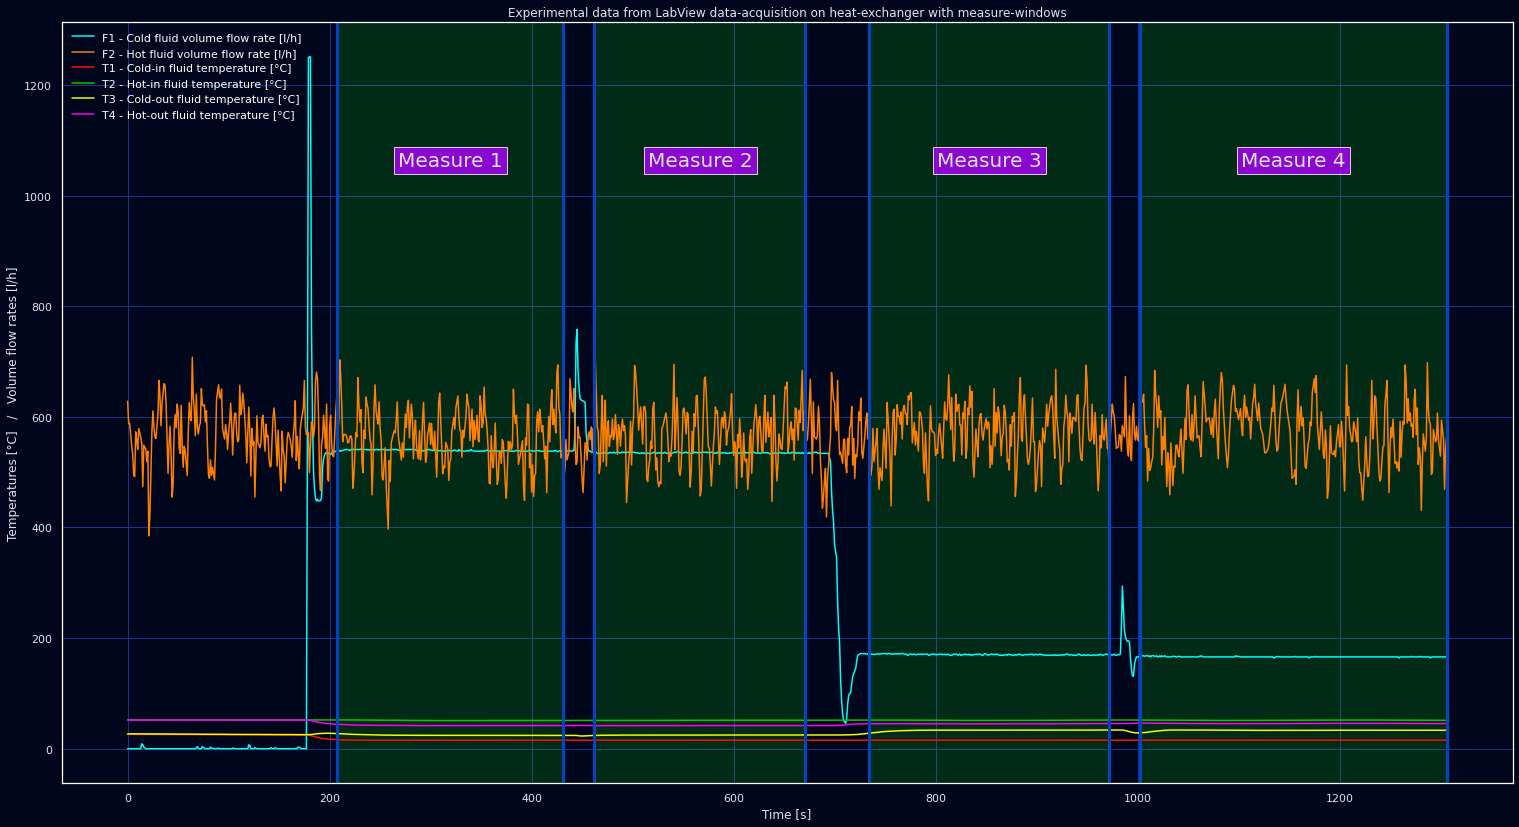
\includegraphics[width=0.8\textwidth]{../final_doc/code_exports/imgs/measures.png}                                        % Size: 100% width of the text
\end{figure}                                                                                                                % Figure-end
\begin{figure}[H]                                                                                                           % Figure-start
  \caption{\textit{Scelta del miglior intervallo dati durante la terza misura (ricerca condizioni stazionarie)}}            % Image caption
  \label{fig:measure1}                                                                                                      % Reference-label to image
  \vspace{3mm}                                                                                                              % Vert space
  \centering                                                                                                                % Center image
  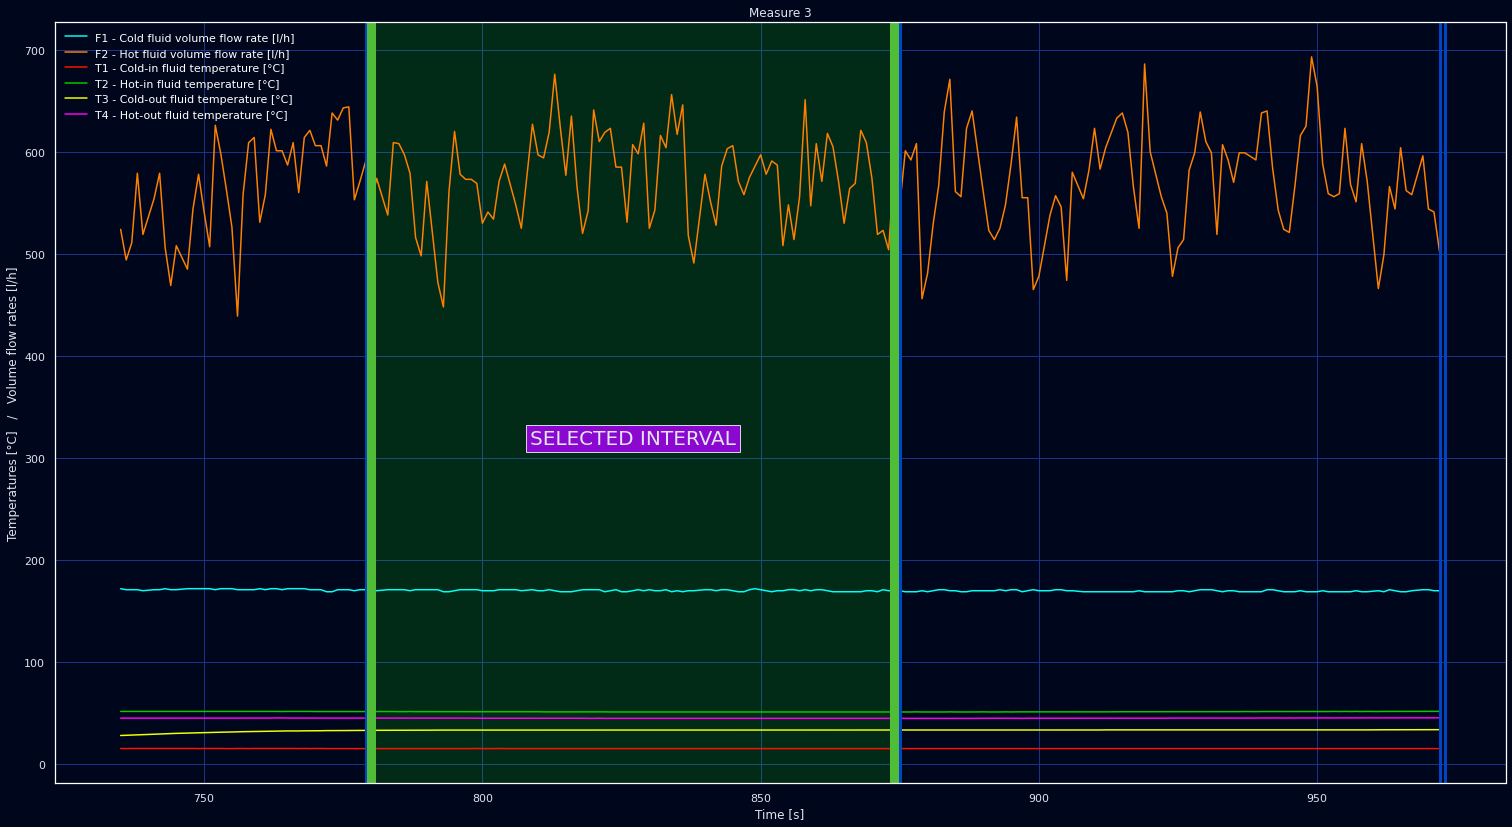
\includegraphics[width=0.8\textwidth]{../final_doc/code_exports/imgs/measure3.png}                                        % Size: 100% width of the text
\end{figure}                                                                                                                % Figure-end
\begin{figure}[H]                                                                                                           % Figure-start
  \caption{\textit{Fitting polinomiale numero di Prandtl acqua (scartato per approssimazione insoddisfacente)}}             % Image caption
  \label{fig:water_fitted_pr}                                                                                               % Reference-label to image
  \vspace{3mm}                                                                                                              % Vert space
  \centering                                                                                                                % Center image
  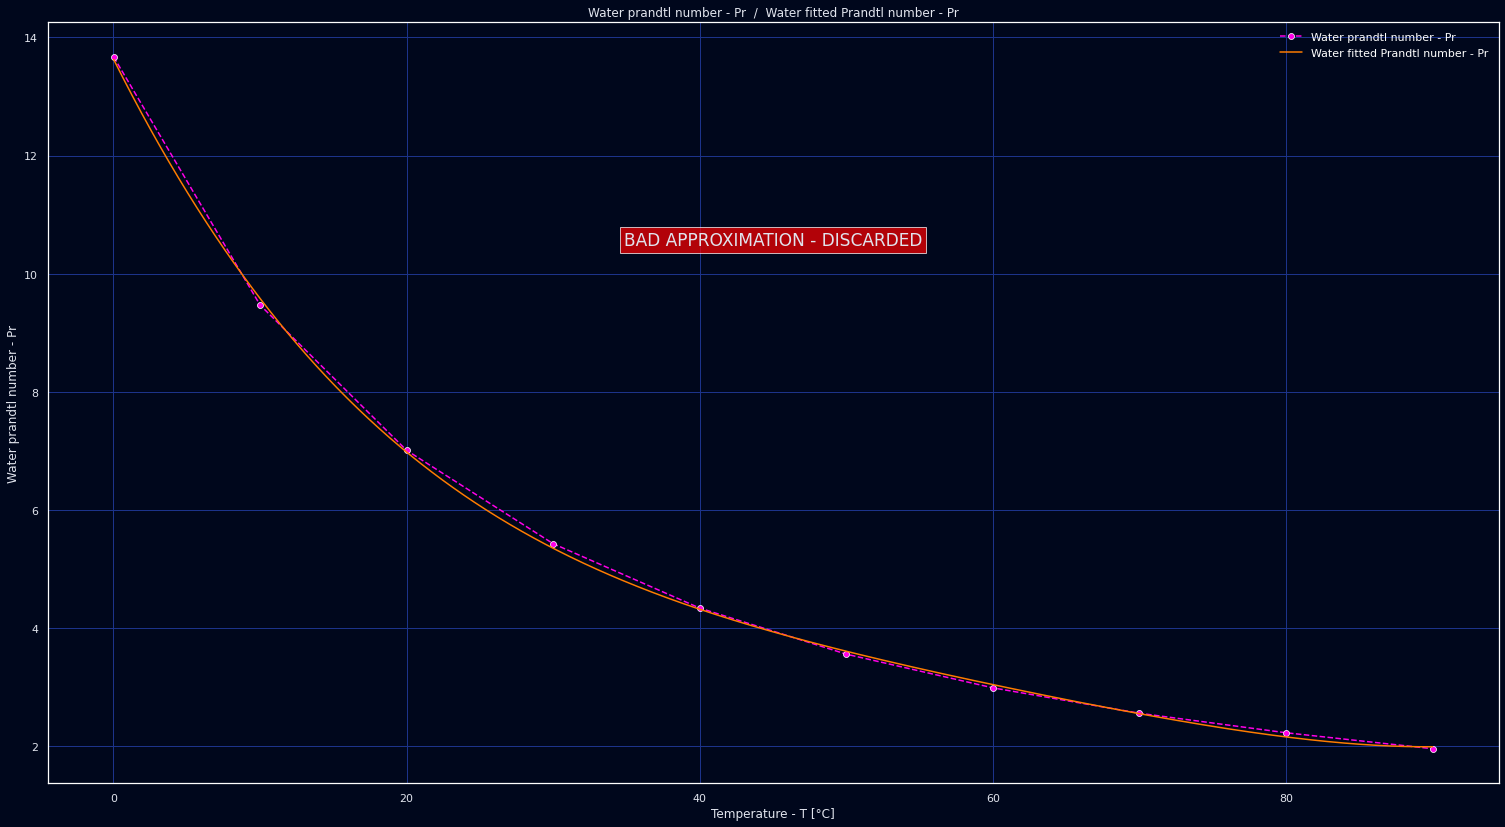
\includegraphics[width=0.8\textwidth]{../final_doc/code_exports/imgs/water_fitted_pr.png}                                 % Size: 100% width of the text
\end{figure}                                                                                                                % Figure-end
\begin{figure}[H]                                                                                                           % Figure-start
  \caption{\textit{Interpolazione polinomiale numero di Prandtl acqua (accettata, buona approssimazione)}}                  % Image caption
  \label{fig:water_intp_pr}                                                                                                 % Reference-label to image
  \vspace{3mm}                                                                                                              % Vert space
  \centering                                                                                                                % Center image
  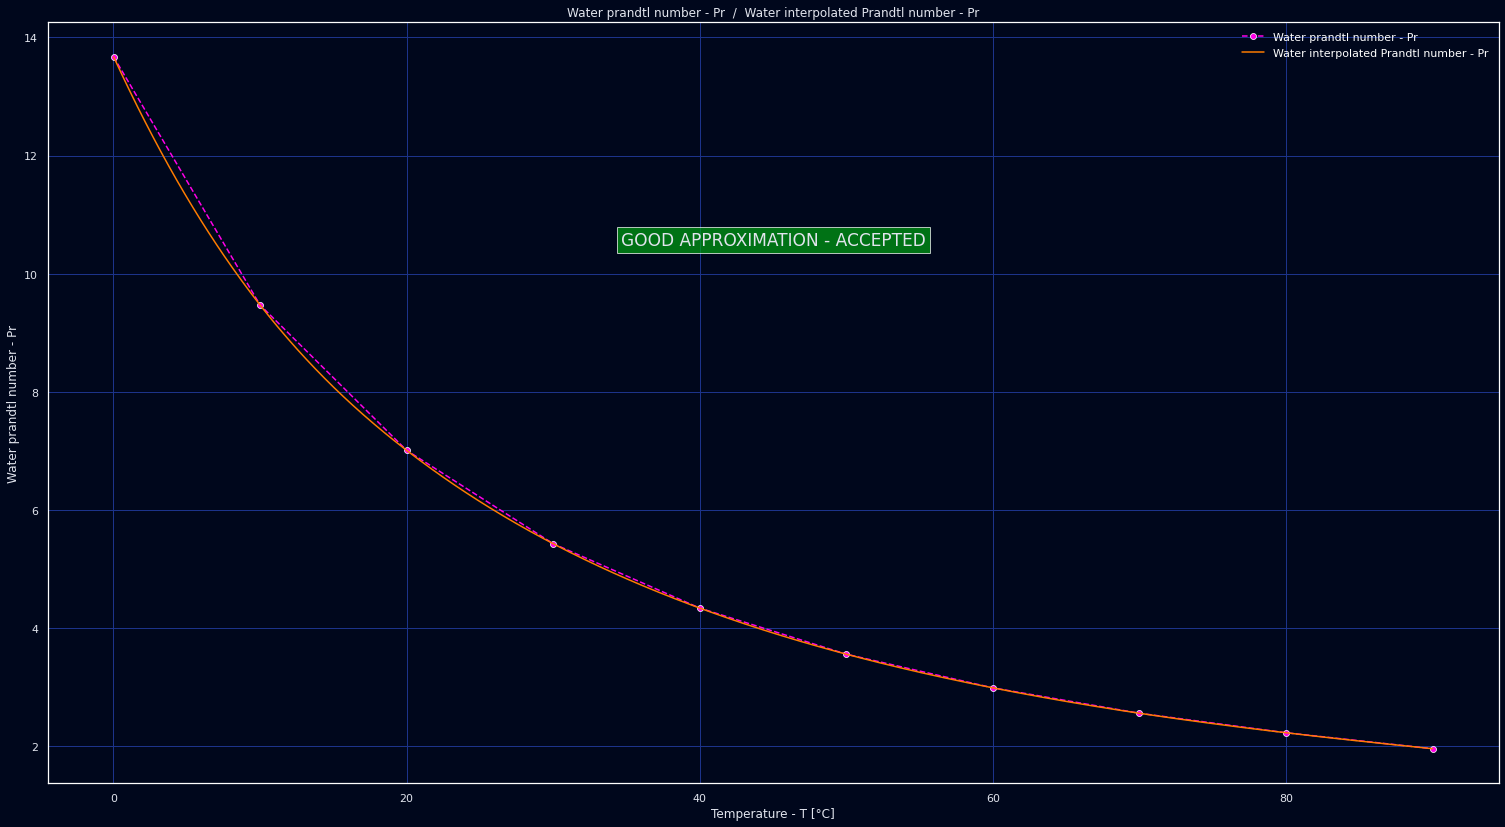
\includegraphics[width=0.8\textwidth]{../final_doc/code_exports/imgs/water_intp_pr.png}                                   % Size: 100% width of the text
\end{figure}                                                                                                                % Figure-end
\begin{figure}[H]                                                                                                           % Figure-start
  \caption{\textit{Alcune temperature nella parte superiore dello scambiatore durante la seconda misura in equi-corrente}}  % Image caption
  \label{fig:temp_trend}                                                                                                    % Reference-label to image
  \vspace{3mm}                                                                                                              % Vert space
  \centering                                                                                                                % Center image
  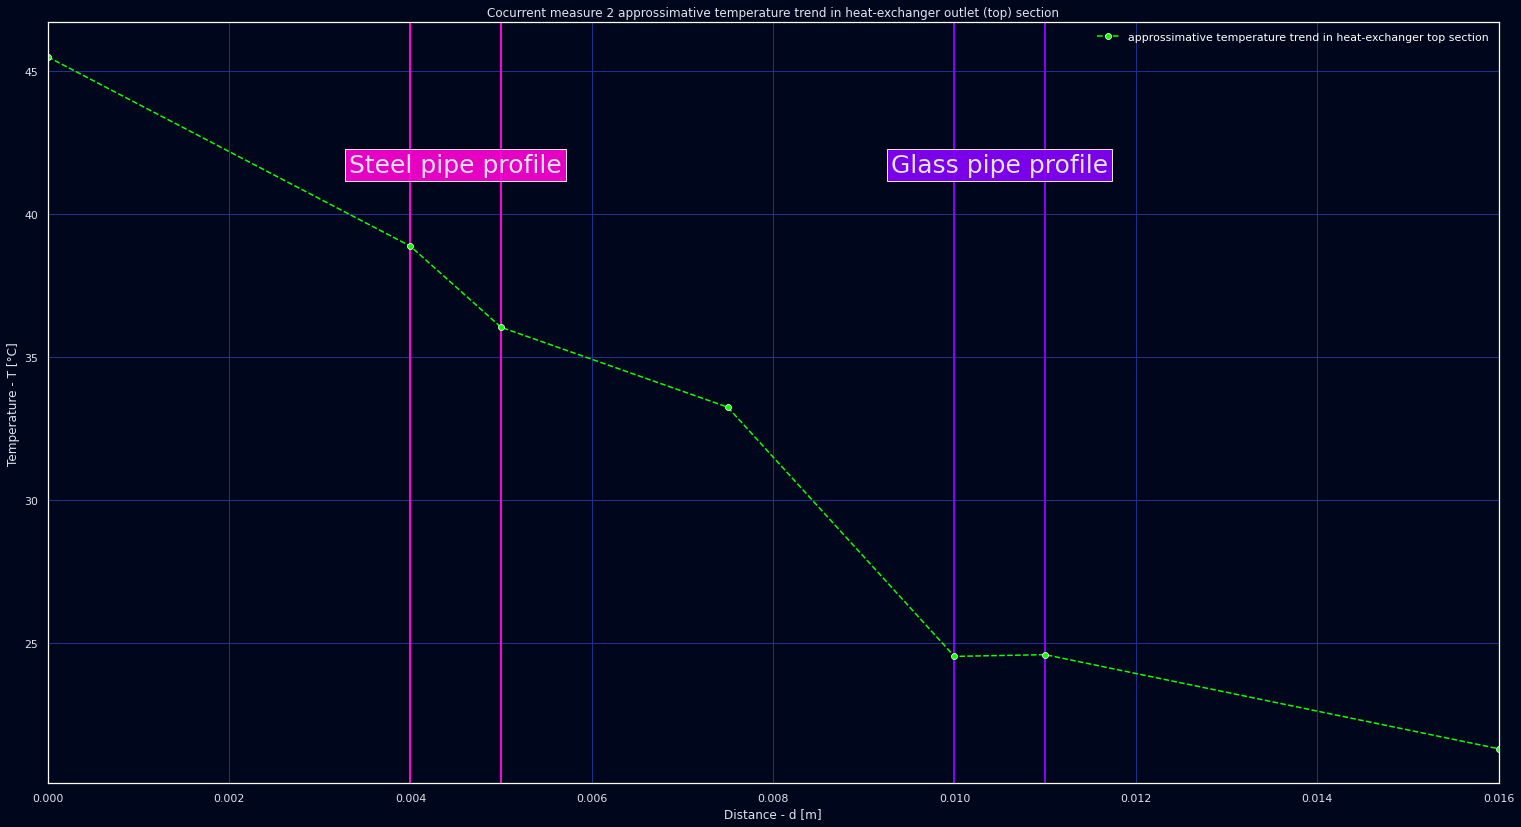
\includegraphics[width=0.8\textwidth]{../final_doc/code_exports/imgs/temp_trend.png}                                      % Size: 100% width of the text
\end{figure}                                                                                                                % Figure-end
\begin{figure}[H]                                                                                                           % Figure-start
  \caption{\textit{Dimensioni scambiatore di calore utilizzate per calcolo dei diametri equivalenti (creata da autocad)}}   % Image caption
  \label{fig:he}                                                                                                            % Reference-label to image
  \vspace{3mm}                                                                                                              % Vert space
  \centering                                                                                                                % Center image
  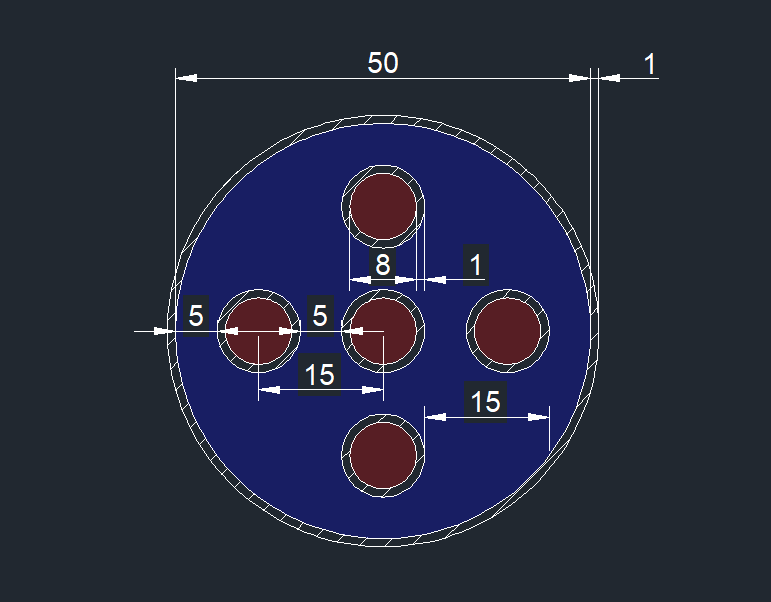
\includegraphics[width=0.8\textwidth]{../final_doc/code_exports/imgs/heat_exchanger.png}                                  % Size: 100% width of the text
\end{figure}                                                                                                                % Figure-end
\clearpage                                                                                                                  % New page

\addcontentsline{toc}{section}{Riferimenti bibliografici}                                                                   % Add bibliography inside table of contents
\bibliography{biblio/references}                                                                                            % Bibliography inclusion (biblio/references.bib)

\end{document}                                                                                                              % End document code

%%%%%%%%%%%%%%%%%%%%%%%%%%%%%%%%%%%%%%
%            DOCUMENT END            %                                                                                      % DOC-END
%%%%%%%%%%%%%%%%%%%%%%%%%%%%%%%%%%%%%%
